\documentclass[aspectratio=1610]{beamer}
\usepackage{hyperref}
\usepackage[T1]{fontenc}

% other packages
\usepackage{latexsym,amsmath,xcolor,multicol,booktabs,calligra}
\usepackage{graphicx,pstricks,listings,stackengine}
\usepackage{ragged2e}
\usepackage[backend=bibtex,sorting=none]{biblatex} % biblatex
\setbeamerfont{footnote}{size=\tiny}
\addbibresource{ref.bib}

\usepackage{lipsum}

\author{Zhouxin Xue, Xuanhang Diao}
\title{Scheduling Beyond CPUs for HPC}
\subtitle{Fan Y, Lan Z, Rich P, et al. \\
\textit{HPDC 19} 
}

\institute{
    School of Biomedical Engineering, \\
    ShanghaiTech University \\
}
\date{14, April}
\usepackage{shanghaitech}

% defs
\def\cmd#1{\texttt{\color{red}\footnotesize $\backslash$#1}}
\def\env#1{\texttt{\color{blue}\footnotesize #1}}
\definecolor{deepblue}{rgb}{0,0,0.5}
\definecolor{deepred}{rgb}{0.6,0,0}
\definecolor{deepgreen}{rgb}{0,0.5,0}
\definecolor{halfgray}{gray}{0.55}

\lstset{
    basicstyle=\ttfamily\small,
    keywordstyle=\bfseries\color{deepblue},
    emphstyle=\ttfamily\color{deepred},    % Custom highlighting style
    stringstyle=\color{deepgreen},
    numbers=left,
    numberstyle=\small\color{halfgray},
    rulesepcolor=\color{red!20!green!20!blue!20},
    frame=shadowbox,
}

\begin{document}

\begin{frame}
    \titlepage
    \begin{figure}[htpb]
        \begin{center}
            
\includegraphics[keepaspectratio, scale=0.2]{pic/ShanghaiTech_Logo.png}
        \end{center}
    \end{figure}
\end{frame}

\section{Background Knowledge}

\begin{frame}{Pareto set}
    A \textbf{Pareto set} is a set of optimal solutions, where no objective can be improved without worsening another objective.
\end{frame}

\begin{frame}{Burst Buffer}
    A \textbf{Burst Buffer} is an intermediate storage layer positioned between compute nodes and parallel file systems (PFS) in high-performance computing (HPC) systems. 
    \begin{itemize}
        \item Absorb the bursty I/O data generated by data-intensive applications.
        \item Built from solid-state drives (SSDs).
        \item Can be either attached to compute nodes as local resources or configured as global resources shared by compute nodes.
    \end{itemize}
\end{frame}

\section{Background and Motivation}

\begin{frame}{Multi-Resource Scheduling}

    \begin{itemize}
        \item HPC systems are equipped with diverse global and local resources.
        \item HPC job scheduler plays a crucial role in efficient use of resources.
    \end{itemize}

    \begin{figure}[htpb]
        \begin{center}
            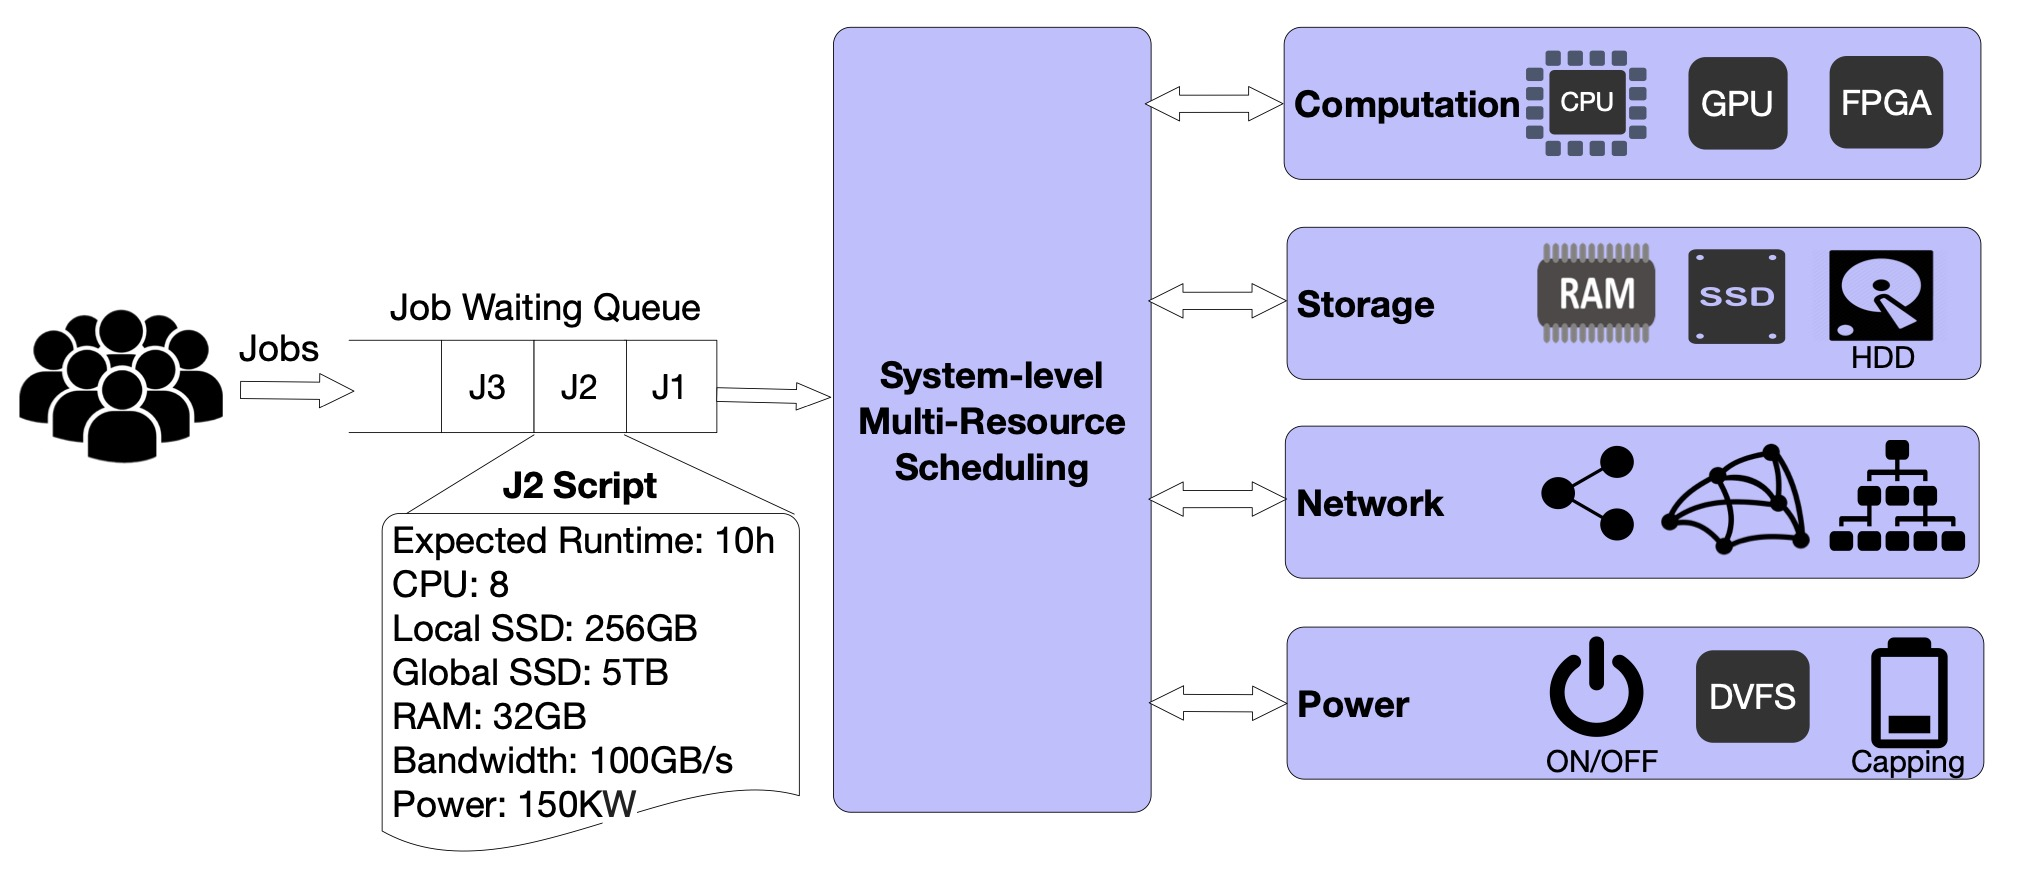
\includegraphics[keepaspectratio, scale=0.12]{pic/sched_with_multi_res.jpeg}
        \end{center}
        \caption{HPC job scheduling problem involves in multiple resources.}
        \label{fig:sched_with_multi_res}
    \end{figure}
   
\end{frame}

\begin{frame}{Limitations of Existing Scheduling Methods}
    
    Existing methods often overlook alternative solutions or optimal resource combinations, leading to under-utilization of resources or poor application performance.
    
    \begin{itemize}
        \item Naive method
        \item Constrained method
        \item Weighted method
        \item Bin packing method
    \end{itemize}
    
\end{frame}

\begin{frame}{Goal}

    The Motivation of the this paper is to improve overall resource utilization and reduce job wait time in HPC systems.

    \begin{itemize}
        \item providing rapid scheduling decisions
        \item minimizing the impact on site policies
        \item ensuring extensibility to accommodate emerging resources
    \end{itemize}
   
\end{frame}

\section{Methodology of BBSched}

\begin{frame}{Window-based Scheduling}
    The idea of window-based scheduling as shown in Fig \ref{fig:BBsched} is that the first $w$ jobs in the job waiting queue get copied into the window.   \\

    This allows our BBsched to consider the site policies and keep the order of the base scheduler as similar as possible.
    \begin{figure}[htpb]
        \begin{center}
            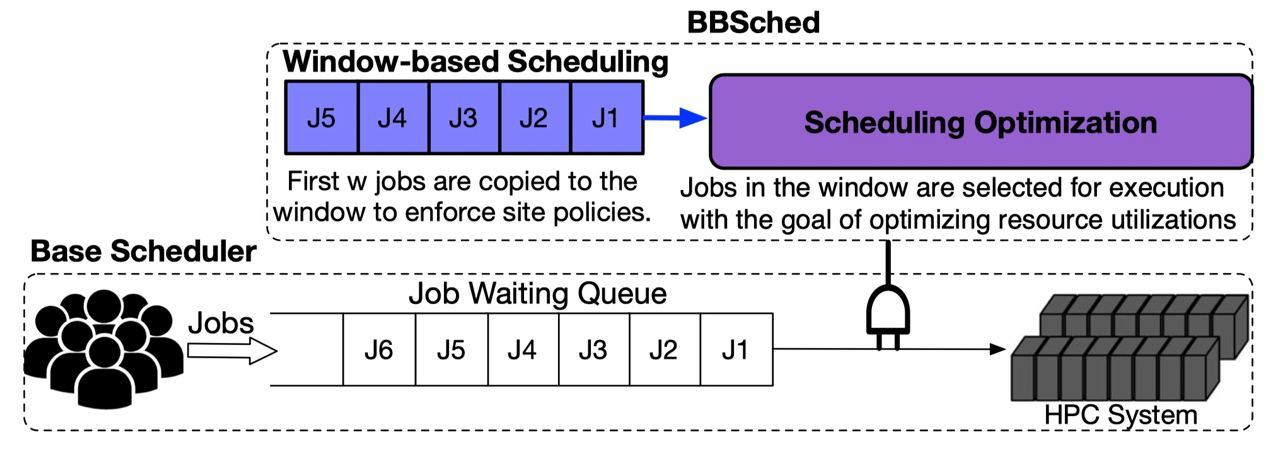
\includegraphics[keepaspectratio, scale=0.2]{pic/BBSched.jpg}
            \caption{The overview of BBsched.}
            \label{fig:BBsched}
        \end{center}
     \end{figure}
\end{frame}

\begin{frame}{MOO Solver}

    Suppose a system has $N$ nodes and burst buffers of total $B$ GB. 
    The amounts of nodes and burst buffers being used are $N_{used}$ and $B_{used}$ respectively.
    Suppose $J = \{J_1 , . . . , J_w \} $is a set of $w$ jobs in the scheduling window. 
    Job $J_i$ requiring $n_i$ nodes and $b_i $GB of burst buffers. \\
    \vspace{10pt}
    The scheduling problem can be transformed into the following MOO: 
    to determine a finite set of Pareto solutions $X$; 
    each Pareto solution $x \in X$ is represented by a binary vector $x = [x_1 , . . . ,x_w ]$, 
    such that $x_i = 1$ if $J_i$ is selected to execute and $x_i = 0$ otherwise. \\
    \vspace{10pt}
    Pareto solution optimizes the following two objectives: \\
    (1) maximize node utilization:  $f_{1}(\boldsymbol{x})=\sum_{i=1}^{w} n_{i} \times x_{w}$ \\
    (2) maximize burst buffer utilization:  $f_{2}(\boldsymbol{x})=\sum_{i=1}^{w} b_{i} \times x_{i}$ \\  
    Formally, the problem can be formulated as:
    $$
    \begin{array}{ll}
    \max & \left(f_{1}(\boldsymbol{x}), f_{2}(\boldsymbol{x})\right) \\
    \text { s.t. } & \sum_{i=1}^{w} n_{i} \times x_{i} \leq N-N_{\text {used }}, \quad x_{i} \in\{0,1\} \\
    & \sum_{i=1}^{w} b_{i} \times x_{i} \leq B-B_{\text {used }}, \quad x_{i} \in\{0,1\}
    \end{array}
    $$

\end{frame}

\begin{frame}{MOO Solver}
    Because this MOO problem is NP-hard, this paper uses a genetic algorithm to approximate the Pareto set (optimal solutions). \\
    \begin{figure}
        \begin{center}
            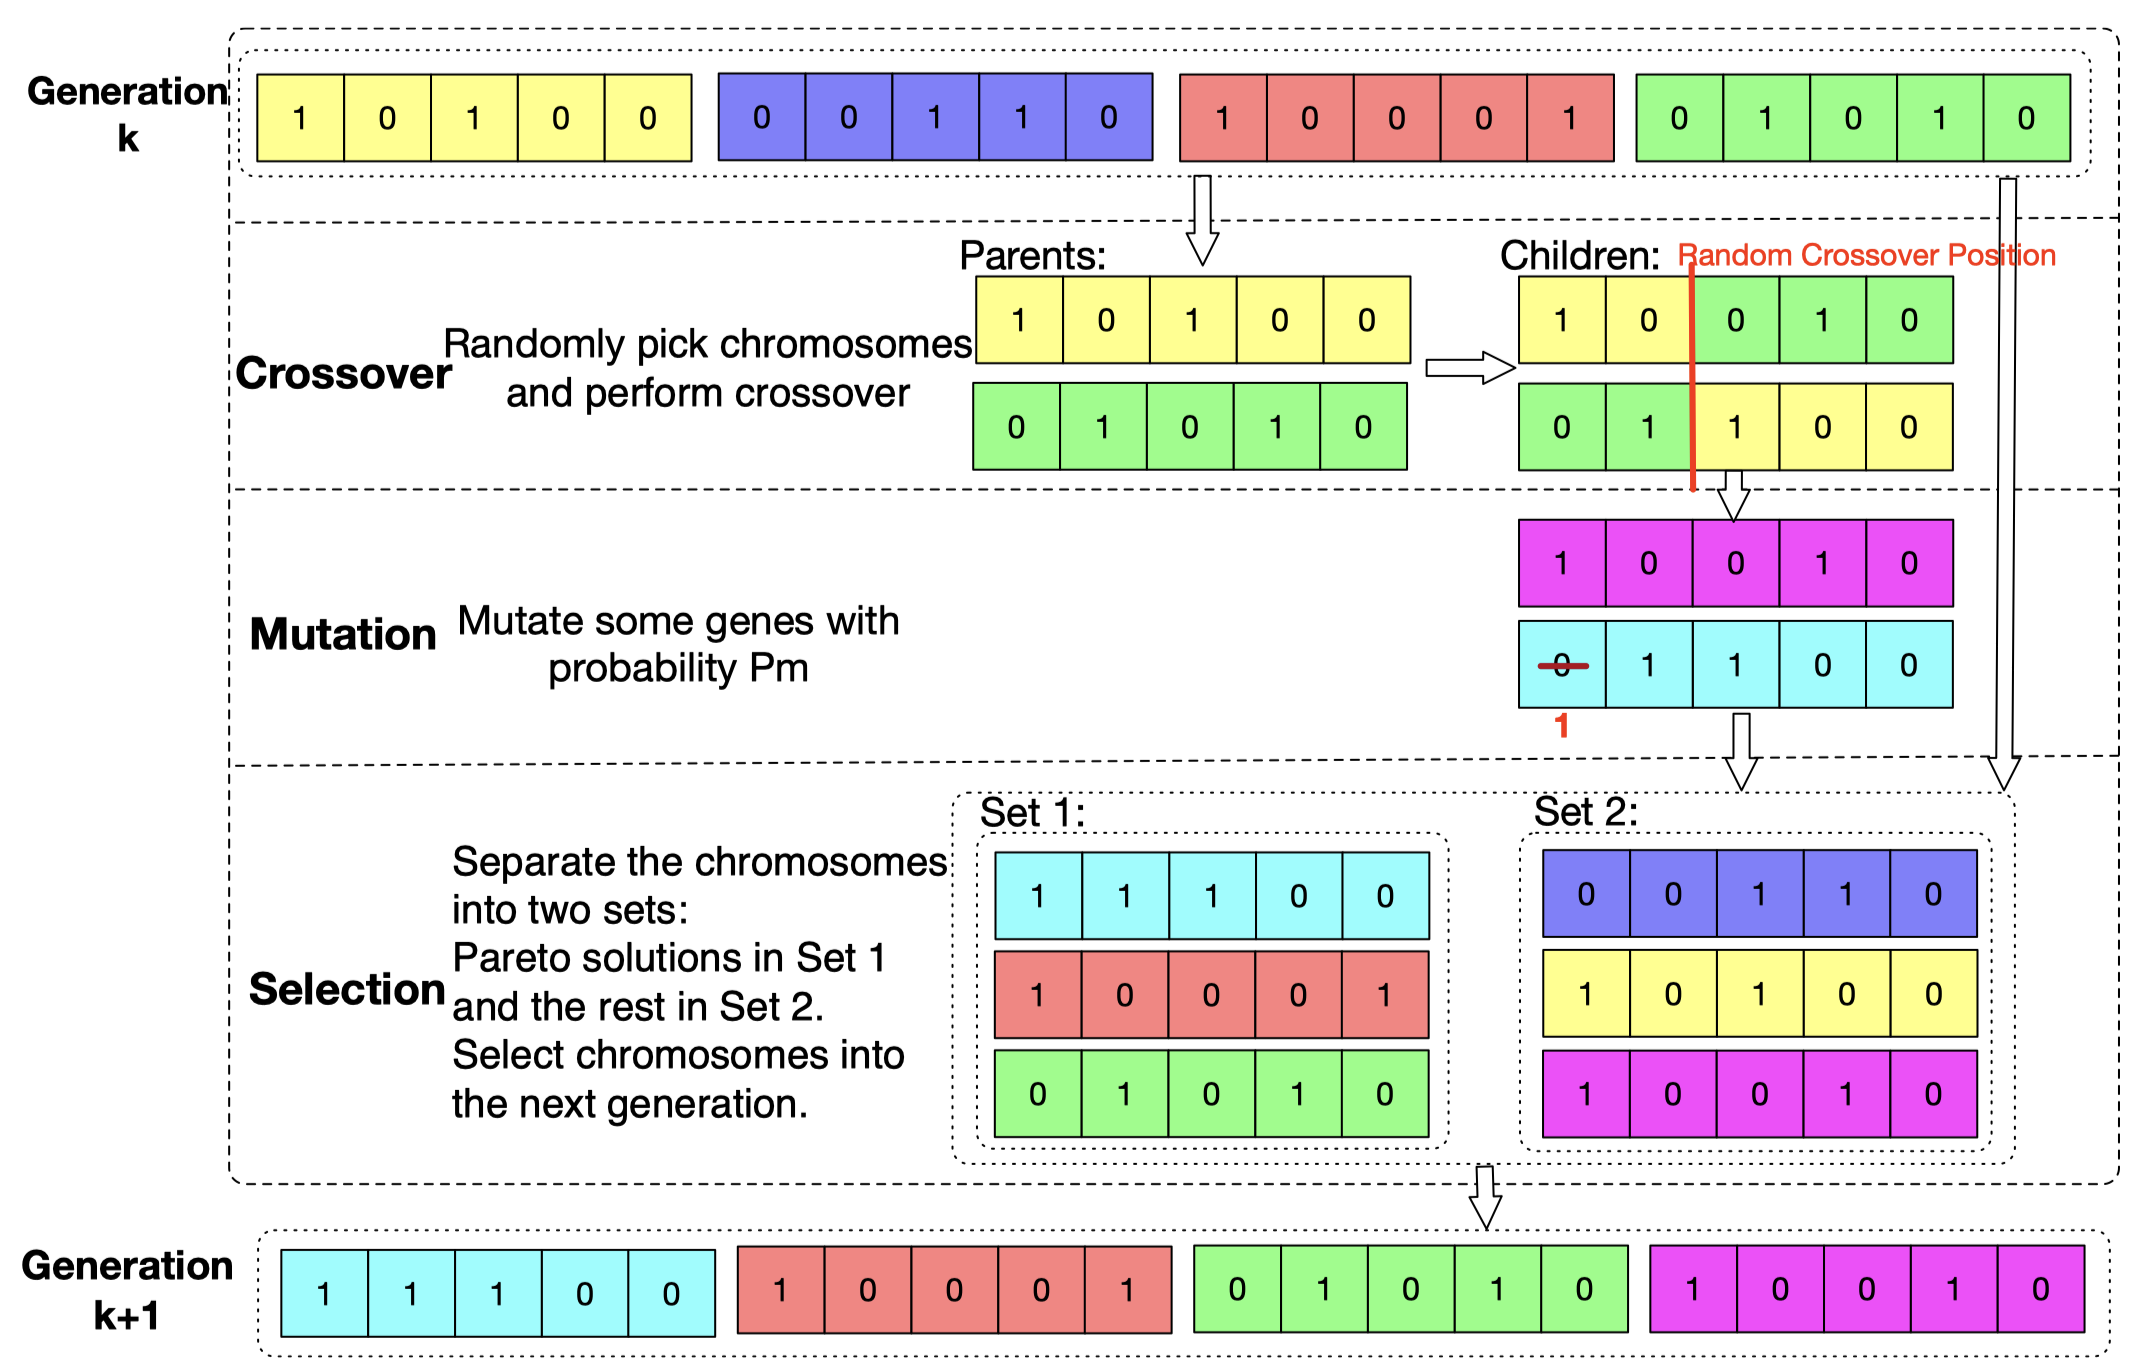
\includegraphics[keepaspectratio, scale=0.18]{pic/genetic.png}
            \caption{MOO solver maintains a population of candidate solutions (4 chromosomes). 
            A chromosome consists of 5 genes, where each gene represents the selection of the job at a specific location in the window and encodes as a binary number: 1 (selected) or 0 (not selected).}
            \label{fig:Genetic_Algorithm}
        \end{center}
    \end{figure}
\end{frame}

\begin{frame}{Decision making}
    The output of the solver is a Pareto set, and a decision maker needs to select one preferred solution. \\
    \vspace{10pt}
    Different HPC facilities may have different site policies and scheduling priorities. \\
    \vspace{10pt}
    System managers may use a site-specific metric for selecting a preferred solution out of the Pareto set. 
\end{frame}
\end{document}